\newcommand{\GO}[1]{\ensuremath{O(#1)}\xspace}
\newcommand{\SO}[1]{\ensuremath{O\tilde\ (#1)}\xspace}
\newcommand{\vect}[1]{\ensuremath{\mathbf{#1}}\xspace}
\newcommand{\mat}[1]{\ensuremath{\mathbf{#1}}\xspace}
%%%%%%%%%%%%%%%%%%%%%%%%%%%%%%%%%%%%%%%%%%%%%%%%%%%%%ùù
%%%%%%%%%%%%%%%%%%%%%%%%%%%%%%%%%%%%%%%%%%%%%%%%%%%%%ùù
\section{Algorithmic aspect}

Solving exactly over the field of rational numbers, requires a careful attention to the size of the numbers being
manipulated. Indeed, rational numbers are represented by a pair of multiprecision integers, a numerator and
denominator. Applying the standard direct methods designed for solving approximately systems with floating point
rational numbers would lead to a blowup in the bitsize of the coefficients, and result in overwelming computation
overheads, with time complexities often not even polynomial.

\subsection{State of the art}
%% \TODO{clarify from the onset that the following paragraph is about
%%   literature, not work done here (right?)}

In a series of algorithmic innovations, summarized in Table~\ref{tab:complexities}, the time complexity for solving exactly a linear system over the rationals has
been reduced to $\SO{n^3}$ or $\SO{n^\omega}$ which is asymptotically as fast as the complexity for solving
approximately using floating point numbers.

First, the use of rational reconstruction makes it possible to recover the rational solution from the solution of the same
system projected into a large enough finite field.
This approach avoids the  swell in the bitsize of the intermediate computations and compute with the arithmetic precision of the output for a total cost of $\GO{n^5}$.
Then, using  multi-modular representation and the Chinese Remainder Theorem, reduces this cost  to $\SO{n^4}$.
This cost, corresponding to the arithmetic complexity of Gaussian elimination multiplied by the bitsize of the output,
is sub-optimal. By better balancing the computation load between numerous arithmetic operation on small bitsize and
few operations on large bitsize, one can hope to further reduce this complexity. This is achieved by $p$-adic lifting
techniques~\cite{Dix82}, reaching a $\SO{n^3}$ time complexity. Improving the complexity for this problem is still a
very active topic: \cite{Sto05} reduced it to $\SO{n^\omega}$ using randomization, and the same
complexity can now be reached deterministically since this year~\cite{BLS19}.



\begin{table}[htb]
\begin{tabular}{lc}
  \toprule
  Method  & Bit complexity \\
  \midrule
  Gauss over $\mathbb{Q}$ & $2^{\GO{n}}$ \\
  Gauss $\mod \text{bound}(sol)$ & $\GO{n^5}$\\
  CRT $\times$ Gauss $\mod p$ & $\SO{n^4}, \SO{n^\omega+1}$\\
  $p$-adic lifting & $\SO{n^3}, \SO{n^\omega}$\\
  \bottomrule
\end{tabular}
\caption{Brief overview of algorithmic innovations for solving linear systems over the rationals}\label{tab:complexities}
\end{table}

While $p$-adic lifting techniques achieve the best complexity for sequential computations, they are unfortunately very
iterative in their structure, and therefore harder to parallelize at a large scale. On the contrary, Chinese remainder
based methods offer an embarrassingly parallel structure, but cost a factor of $n$ more. We have therefore chosen to
explore both approaches which will be described in the following subsections.
%%%%%%%%%%%%%%%%%%%%%%%%%%%%%%%%%%%%%%%%%%%%%%%%%%%%%ùù
\subsection{The Chinese remainder approach}

We recall here the principle of the Chinese Remainder based rational solver:
the linear system over the integers is reduced modulo a series of prime numbers. Each of these systems can then be solved
independently, therefore exposing a large degree of parallelism. The rational solution can then be recovered in two
phases by a Chinese remainder reconstruction followed by a vector rational reconstruction.

\begin{algorithm}[htb]
  \caption{Chinese Remainder based rational solver}\label{alg:CRTRS}
  \begin{algorithmic}[1]
    \Require{$\mat{A}\in \mathbb{Z}^{n\times n},\vect{b}\in\mathbb{Z}^n$}
    \Ensure{$\vect{x}$ such that $\mat{A}\vect{x}=\vect{b}$}
    \State $N,D \leftarrow \text{SolutionBounds}(\mat{A},b)$
    \State Pick $\ell$ primes $p_1,\dots, p_\ell$ such that $\prod_{i=1}^\ell p_i \geq 2ND$
    \For{$i\leftarrow 1\dots \ell$}
    \State\label{lin:CRT:RNSA} $\mat{A}^{(i)} \leftarrow \mat{A}\mod p_i$
    \State\label{lin:CRT:RNSb} $\vect{b}^{(i)} \leftarrow \vect{b}\mod p_i$
    \State\label{lin:CRT:solve} $\vect{x}^{(i)} \leftarrow (\mat{A}^{(i)})^{-1} \vect{b}^{(i)} \mod p_i$
    \EndFor
  \State\label{lin:CRT:CRT} $\vect{y} \leftarrow \texttt{ChineseRemainder}(\vect{y}^{(1)},p_1,\dots, \vect{y}^{(\ell)},p_\ell)$
  \State\label{lin:CRT:RR} $\vect{x},d\leftarrow \texttt{VectorRationalReconstruction}(\vect{y},\prod_{i=1}^\ell p_i)$
  \State \Return $\vect{x}/d$
\end{algorithmic}
\end{algorithm}

In sequential versions of this algorithm, the Chinese remainder and rational reconstruction can be performed on the fly
after each iteration, in order to detect stabilization and allow to terminate the loop earlier than what the possibily
pessimistic bound on the solution requires. In parallel, this would generate depency between the parallel tasks and we
thus chose to disable this feature.


%%%%%%%%%%%%%%%%%%%%%%%%%%%%%%%%%%%%%%%%%%%%%%%%%%%%%ùù
\subsection{The $p$-adic lifting approach}

The $p$-adic lifting approach, developped in~\cite{Dix82} is based on a Newton iteration to compute iteratively the
digits in the $p$-adic expansion of the solution vector. This algorithm manages to reduce the cost of Chinese Remaindering
by balancing two types of operations: expensive linear algebra (matrix inverse or LU decomposition) is
perfomed only once over in small precision (a finite field) while the high precision part of the computation is
contained in a sequence of less expensive linear algebra operations (matrix-vector products).
%\begin{algorithm}[htb]
%  \caption{$p$-adic lifting based rational solver}
%  \begin{algorithmic}[1]
%    \Require{$\mat{A}\in \mathbb{Z}^{n\times n},\vect{b}\in\mathbb{Z}^n$}
%    \Ensure{$\vect{x}$ such that $\mat{A}\vect{x}=\vect{b}$}
%    \State $N,D \leftarrow \text{SolutionBounds}(\mat{A},b)$
%    \State Pick a prime $p$. Let $k$ such that $p^k \geq 2ND$
%    \State $\mat{B}\leftarrow \mat{A}^{-1} \mod p$
%    \State $\vect{r}\leftarrow \vect{b}$
%    \For{$i\leftarrow 0\dots k$}
%    \State $\vect{c}^{(i)}  \leftarrow \mat{B} \vect{r} \mod p_i$
%    \State $\vect{r} \leftarrow  \frac{\vect{r} - \mat{A}\vect{x_i}}{p}$
%    \EndFor
%    \State $\vect{y} \leftarrow \sum_{i=0}^{k-1} \vect{c}^{(i)} p^i$
%    \State $\vect{x},d\leftarrow \texttt{VectorRationalReconstruction(\vect{y})}$
%  \State \Return $\vect{x}/d$
%\end{algorithmic}
%\end{algorithm}

However, the strongly iterative structure of this algorithm makes it both harder to parallelize and less cache
efficient.
In \cite{ChSt05}, Storjohann and Chen devised a way to improve the cache efficiency thanks to a hybrid combination of
$p$-adic lifting and Chinese remainder techniques.
This led to a multi-modular (or RNS, residue number system) $p$-adic
lifting.
We further improve this variant in several ways to deliver a parallel
RNS $p$-adic lifting solver. The novel
Algorithm~\ref{alg:ParMultiModSolve} reflects these improvements with
the two following salient features:
\begin{enumerate}
\item The costly updates in the main loop of \cite{ChSt05} were
  performed via matrix-vector arbitrary precision multiplications over
  the integers with a second RNS basis.
  We instead gather those updates in order to perform instead a
  matrix-matrix multiplication.
  This can be seen in line~\ref{lin:ZGEMM} of
  Algorithm~\ref{alg:ParMultiModSolve}.
\item We mix this algorithm with the parallel RNS improvement
  of~\cite{DGLS18} and restrict the second RNS basis to primes
  individually larger than the
  multi-modular high-level ones in order to speed up the RNS/integer
  conversions.
\end{enumerate}

%\begin{algorithm}[htb]
%  \caption{Multi-modular $p$-adic rational solver}\label{alg:ChSt}
%  \begin{algorithmic}[1]
%    \Require{$\mat{A}\in \mathbb{Z}^{n\times n},\vect{b}\in\mathbb{Z}^n$, $\ell$ a parameter}
%    \Ensure{$\vect{x}$ such that $\mat{A}\vect{x}=\vect{b}$}
%    \State $N,D \leftarrow \text{SolutionBounds}(\mat{A},b)$
%    \State Pick $\ell$ primes $p_1,\dots, p_\ell$ and let $k$ such that $\prod_{i=1}^\ell p_i^k \geq 2ND$
%    \For{$i\leftarrow 1 \dots \ell$}
%      \State $B_i \leftarrow  A^{-1} \mod p_i$
%      \State $\vect{r}^{(i,0)}\leftarrow \vect{b} \mod p_i$
%    \EndFor
%    \For{$j\leftarrow 0\dots k-1$}
%    \For{$i\leftarrow 1\dots\ell$}
%    \State $\vect{c}^{(i,j)}  \leftarrow \mat{B_i} \vect{r_i} \mod p_i$
%    \State $(\vect{Q}^{(i,j)},\vect{R}^{(i,j)}) \leftarrow
%    \texttt{divmod}(\vect{r}^{(i,j)},p_i)$\hfill\Comment{$\vect{r}^{(i,j)} = p_i \vect{Q}^{(i,j)} + \vect{R}^{(i,j)}$}
%    \State $\vect{r}^{(i,j+1)} \leftarrow\vect{Q}^{(i,j)}+\frac{\vect{R}^{(i,j)} - \mat{A}\vect{c}^{(i,j)}}{p_i}$ \hfill\Comment{$\frac{\vect{r}^{(i,j)} - \mat{A}\vect{c}^{(i,j)}}{p_i}$}
%    \EndFor
%    \EndFor
%    \For{$i\leftarrow 1\dots\ell$}
%    \State $\vect{y}^{(i)} \leftarrow \sum_{j=0}^{k-1} \vect{c}^{(i,j)} p_i^j$
%    \EndFor
%    \State $\vect{y} \leftarrow \texttt{ParallelChineseRemainder}(\vect{y}^{(1)},p_1^k,\dots, \vect{y}^{(\ell)},p_\ell^k)$
%    \State $\vect{x},d\leftarrow \texttt{VectorRationalReconstruction}(\vect{y},\prod_{i=1}^\ell p_i^k )$
%  \State \Return $\vect{x}/d$
%\end{algorithmic}
%\end{algorithm}

\begin{algorithm}[htb]
  \caption{Parallel multi-modular $p$-adic rational solver}\label{alg:ParMultiModSolve}
  \begin{algorithmic}[1]
    \Require{$\mat{A}\in \mathbb{Z}^{n\times n},\vect{b}\in\mathbb{Z}^n$, $\ell$ a parameter}
    \Ensure{$\vect{x}$ such that $\mat{A}\vect{x}=\vect{b}$}
    \State $N,D \leftarrow \text{SolutionBounds}(\mat{A},b)$
    \State Pick $\ell$ primes $p_1,\dots, p_\ell$ and let $k$ such that $\prod_{i=1}^\ell p_i^k \geq 2ND$
    \For{$i\leftarrow 1 \dots \ell$ in parallel}
      \State\label{lin:INV} $B_i \leftarrow  A^{-1} \mod p_i$
      \State $\vect{r}^{(i)}\leftarrow \vect{b} \mod p_i$
      \State $\vect{y}^{(i)} \leftarrow 0$
    \EndFor
    \State Pick primes $q_1,\dots, q_\tau$, all $>\max_i\{p_i\}$, such
    that $\prod_{s=1}^\tau q_s \geq n||A||_\infty$
    \For{$j\leftarrow 0\dots k-1$}
    \For{$i\leftarrow 1\dots\ell$ in parallel}
    \State $(\vect{\phi}^{(i)},\vect{\rho}^{(i)}) \leftarrow
    \texttt{divmod}(\vect{r}^{(i)},p_i)$\Comment{$\vect{r}^{(i)} = p_i \vect{\phi}^{(i)} + \vect{\rho}^{(i)}$}
    \State\label{lin:GEMV} $\vect{c}^{(i)}  \leftarrow \mat{B_i} \vect{\rho}^{(i)} \mod p_i$
    \State $\vect{y}^{(i)} \leftarrow \vect{y}^{(i)} + \vect{c}^{(i)} p_i^j$
%    \State $\vect{r}^{(i,j+1)} \leftarrow\vect{\phi}^{(i,j)}+\frac{\vect{\rho}^{(i,j)} - \mat{A}\vect{c}^{(i,j)}}{p_i}$ \Comment{$\frac{\vect{r}^{(i,j)} - \mat{A}\vect{c}^{(i,j)}}{p_i}$}
    \EndFor
\newline{\Comment{Now compute simultaneously all the updates $\frac{\vect{r}^{(i)} -
      \mat{A}\vect{c}^{(i)}}{p_i}$  in parallel:}}
    \State Gather
    $\mat{R}\leftarrow\left[\begin{array}{ccc}\vect{\rho}^{(1)}&\ldots&\vect{\rho}^{(\ell)}\end{array}\right]$
    and $\mat{C}\leftarrow\left[\begin{array}{ccc}\vect{c}^{(1)}&\ldots&\vect{c}^{(\ell)}\end{array}\right]$
    \State\label{lin:ZGEMM}
    $\mat{V}\leftarrow\mat{R}-\mat{A}\cdot\mat{C}$\Comment{Parallel RNS with $q_1,\dots, q_\tau$}
    \For{$i\leftarrow 1\dots\ell$ in parallel}
    \State $\vect{r}^{(i)}
    \leftarrow\vect{\phi}^{(i)}+\frac{\vect{V_{*,i}}}{p_i}$\Comment{Multiply by $(p_i^{-1}{\mod{q_s}})$ in RNS, then reconvert to $\mathbb{Z}^n$}
    \EndFor
    \EndFor
    \State $\vect{y} \leftarrow \texttt{ParallelChineseRemainder}(\vect{y}^{(1)},p_1^k,\dots, \vect{y}^{(\ell)},p_\ell^k)$
    \State $\vect{x},d\leftarrow \texttt{VectorRationalReconstruction}(\vect{y},\prod_{i=1}^\ell p_i^k )$
  \State \Return $\vect{x}/d$
\end{algorithmic}
\end{algorithm}

%%%%%%%%%%%%%%%%%%%%%%%%%%%%%%%%%%%%%%%%%%%%%%%%%%%%%ùù
%%%%%%%%%%%%%%%%%%%%%%%%%%%%%%%%%%%%%%%%%%%%%%%%%%%%%ùù
\section{High performance parallelization}

The implementations referred to for this deliverable are made in the \Linbox library.


%%%%%%%%%%%%%%%%%%%%%%%%%%%%%%%%%%%%%%%%%%%%%%%%%%%%%ùù
\subsection{MPI based Chinese remainder algorithm}

\begin{itemize}
\item  Full MPI vs Hybrid MPI-OMP (memory savings).
\item Asymptotically fast vector Chinese remainder $\Rightarrow$ not a bottleneck anymore
\end{itemize}

\TODO{Pretty convincing figure about scaling factors! Maybe add a line
  representing what a perfect parallelisation would achieve for
  comparison? How comes that the size of the matrix barely matters?}

We first report on the implementation of the parallelization of
Algorithm~\ref{alg:CRTRS} with different matrix dimensions and entry
bitsize. 
On a cluster where each node is equipped
with $2{\times}16$ Intel Gold-6130 @2.1Ghz cores, we obtain the
timings reported in
Figure~\ref{fig:mpi_histo}.
This is for instance a speed up of about $160$ on $8$ nodes.

\begin{figure}[htb]
\begin{center}
  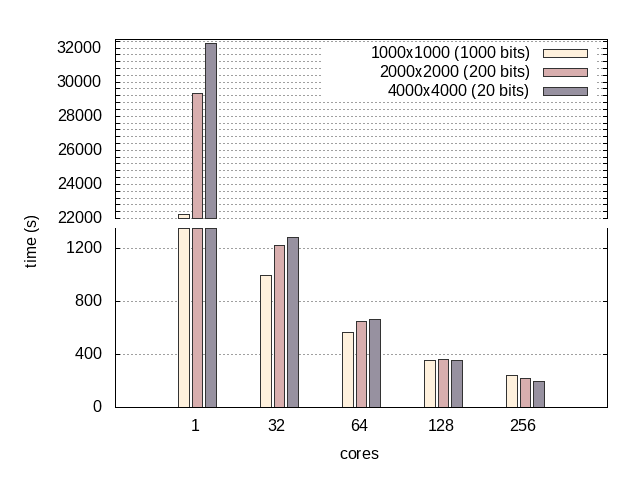
\includegraphics[width=.8\textwidth]{nodes_histogram}
\end{center}
\caption{MPI-Chinese Remainder based rational solver.}\label{fig:mpi_histo}
\end{figure}

The parallelization here is performed only on the main loop,
that is lines~\ref{lin:CRT:RNSA} and~\ref{lin:CRT:RNSb} (RNS) and
line~\ref{lin:CRT:solve} (Solve), whereas the Chinese remaindering
(line~\ref{lin:CRT:CRT} -- CRT) 
and the rational reconstruction (line~\ref{lin:CRT:RR} -- RR) are
performed on a single core. 
Indeed, Table~\ref{tab:MPICRT}, shows the details of the obtained
timings and we see that the Wall time of these two latter parts is not
dominating.


\begin{table}[htb]
\renewcommand{\arraystretch}{1.1}
\begin{tabular}{rrrrrrrrr}
\hline
\multirow{2}{*}{Cores} & \multirow{2}{*}{N}& \multirow{2}{*}{Bitsize}
& \multirow{2}{*}{$\ell$}& RNS & Solve & CRT& RR & Total \\
 & &  & & cpu (s) & cpu (s) & Wall (s)& Wall (s) & Wall (s) \\
\hline
 64  & 1000 & 1000 & 91364 & 11537.1 & 17080.8 & 67.4 & 69.6 & 619.6 \\
 64  & 2000 & 200& 37362 & 6740.0 & 31138.3 & 50.1 & 24.9 & 702.7 \\
 64  & 4000 & 20 & 9450& 2702.9 & 39037.1 & 19.6 & 6.9& 711.9 \\
 128 & 1000 & 1000 & 91364 & 11536.6 & 17136.8 & 67.6 & 71.1 & 398.4 \\
 128 & 2000 & 200& 37362 & 6811.4 & 31193.5 & 50.4 & 25.4& 401.7 \\
 128 & 4000 & 20 & 9450& 2733.1 & 39307.9 & 21.1 & 7.2& 379.3 \\
 256 & 1000 & 1000 & 91364 & 11565.7 & 17138.2 & 70.2 & 73.5& 290.8 \\
 256 & 2000 & 200& 37362 & 6814.9 & 31245.4 & 51.0 & 25.5 & 253.4 \\
 256 & 4000 & 20 & 9450& 2738.3 & 39405.1 & 19.1 & 6.9& 209.9 \\
\hline
\vspace{0pt}
\end{tabular}
\caption{Respective timings of the steps of the MPI CRT}\label{tab:MPICRT}
\end{table}

We also report in Table~\ref{tab:HybridMPIOMP} on some prototype
hybrid MPI/OpenMP implementation where on each node we switch to use
SMP parallelism with OpenMP instead of having MPI handling also the
in-node parallelism. On this particular cluster OpenMP is, for some
unkown reason, much slower than MPI and therefore our Hybrid algorithm
is slower than the pure MPI implementation. Nonetheless this hybrid
implementation allows to not duplicate the data within each node and
therefore enables the solution of much larger matrices 

\begin{table}[htb]
\renewcommand{\arraystretch}{1.1}
\begin{tabular}{rrrrrr}
\hline
 Nodes & Threads & Usertime & Realtime & N     & Bitsize\\
\hline
 2     & 1 & 423.6  & 425.5  & 1000  & 1000 \\
 2     & 16 & 877.1    & 880.2  & 1000  & 1000 \\
 2     & 1 & 432.3  & 434.4  & 2000  & 200  \\
 2     & 16 & 810.1  & 812.9  & 2000  & 200  \\
 2     & 1 & 352.5  & 354.0  & 4000  & 20   \\
 2     & 16 & 863.2  & 866.2  & 4000  & 20   \\
 4     & 1 & 301.0  & 302.4  & 1000  & 1000 \\
 4     & 16 & 517.4  & 519.5  & 1000  & 1000 \\
 4     & 1 & 283.5  & 285.2  & 2000  & 200  \\
 4     & 16 & 420.2  & 422.0  & 2000  & 200  \\
 4     & 1 & 239.4  & 240.6  & 4000  & 20   \\
 4     & 16 & 422.0  & 422.7  & 4000  & 20   \\
 6     & 1 &  - & -  & 10000 & 40   \\
 6     & 16 & 11891.4  & 12026.3  & 10000 & 40   \\
 8     & 1 & 246.9    & 248.4  & 1000  & 1000 \\
 8     & 16 & 415.2  & 417.0  & 1000  & 1000 \\
 8     & 1 & 240.5  & 242.0   & 2000  & 200  \\
 8     & 16 & 299.2  & 300.8  & 2000  & 200  \\
 8     & 1 & 184.5  & 185.4  & 4000  & 20   \\
 8     & 16 & 324.2  & 325.6  & 4000  & 20   \\
 8     & 1 &  - & -  & 10000 & 100  \\
 8     & 16 & 21184.2  & 21443.8  & 10000 & 100  \\
\hline
\vspace{0pt}
\end{tabular}
\caption{Combined MPI/OMP prototyping}\label{tab:HybridMPIOMP}
\end{table}





%%%%%%%%%%%%%%%%%%%%%%%%%%%%%%%%%%%%%%%%%%%%%%%%%%%%%ùù
\subsection{A multicore $p$-adic lifting}
Thanks to our implementation of Algorithm~\ref{alg:ParMultiModSolve},
we obtain improvements on arbitrary precision parallel rational
solving.
All the experiments in this Section were obtained on a single machine
equipped with $4{\times}18$ E7-8860v4 cores @2.2Ghz.


Roughly, the dominant costs of Algorithm~\ref{alg:ParMultiModSolve}
are within lines~\ref{lin:INV}, \ref{lin:MVmod} and~\ref{lin:MMZ},
which we will denote by the INV (matrix inversion), MVmod
(matrix-vector iteration) and MMZ (matrix-matrix multiplication over
$\mathbb{Z}$).
Their respective costs are given by $\GO{\ell\cdot{}n^\omega}$,
$\GO{k\ell\cdot{}n^2}$ and $\GO{k\cdot{}n^2\ell^{\omega-1}}$,
where $\ell$ is the parameter and $k\ell\approx n \cdot
\frac{\texttt{bitsize}}{\log_2(p)}$ is a constant for any $\ell$.

Thus we see that by increasing $\ell$ we increase the overall number
of operations, but the hope is to trade some slow operations of MMZ
for some very fast operations of INV.
We also see that the dominant cost should remain unchanged within MVmod, but
that by increasing $\ell$ we increase the potential for
parallelism.

This analysis is backed up by experiments as we show in the following.
%
First, the technique of the double RNS basis, combined with the
gathering of updates is shown, in sequential, in
Figures~\ref{fig:rnsdixon_seqprimescount}
and~\ref{fig:rnsdixon_seqbitsize}. We see that by extending $\ell$
(``primes'' is the Figures), we increase the overall work but this
can pay at different thresholds for different matrix dimensions and
bitsizes. In sequential we can see some $30\%$ gains on a single core,
even for small matrices.


\begin{figure}[htb]
\begin{center}
  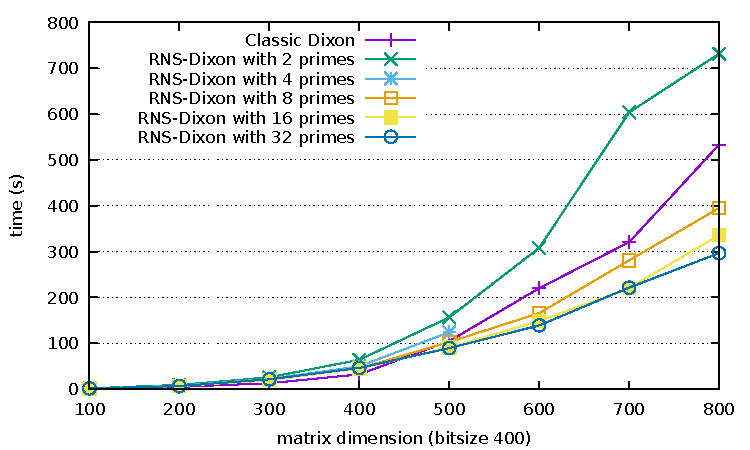
\includegraphics[width=.8\textwidth]{Pictures/RNSDixon/sequential-primesCount}
\end{center}
\caption{Sequential RNS Dixon with fixed bitsize.}\label{fig:rnsdixon_seqprimescount}
\end{figure}
\begin{figure}[htb]
\begin{center}
  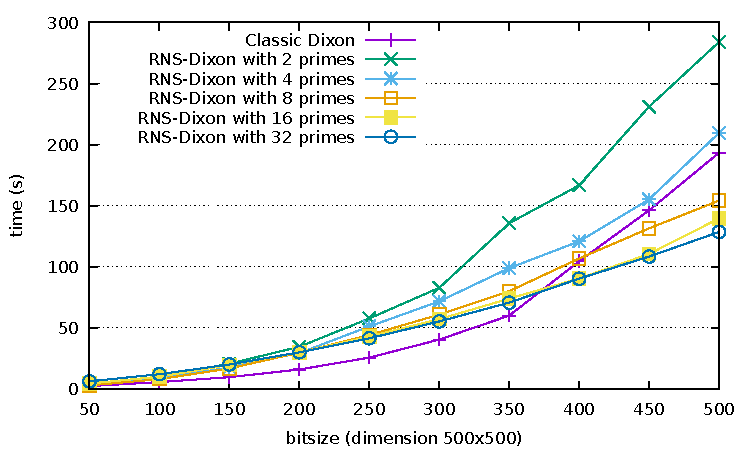
\includegraphics[width=.8\textwidth]{Pictures/RNSDixon/sequential-bitsize}
\end{center}
\caption{Sequential RNS Dixon with fixed matrix dimension.}\label{fig:rnsdixon_seqbitsize}
\end{figure}

Now in parallel we obtain good speed-up, as shown in
Figures~\ref{fig:rnsdixon_parallel_threads}
and~\ref{fig:rnsdixon_parallel}. Indeed, there, we see that the
overall work increases with the increase of $\ell$ (see the top
histograms in Figure~\ref{fig:rnsdixon_parallel}).
But this increase is negligible when the matrix size is larger (almost
no more ``red'' in the bottom histogram), and the parallelization pays
of ($9.6$ speed-up for our new Algorithm with $16$ cores in the bottom
histogram).

\begin{figure}[htb]
\begin{center}
  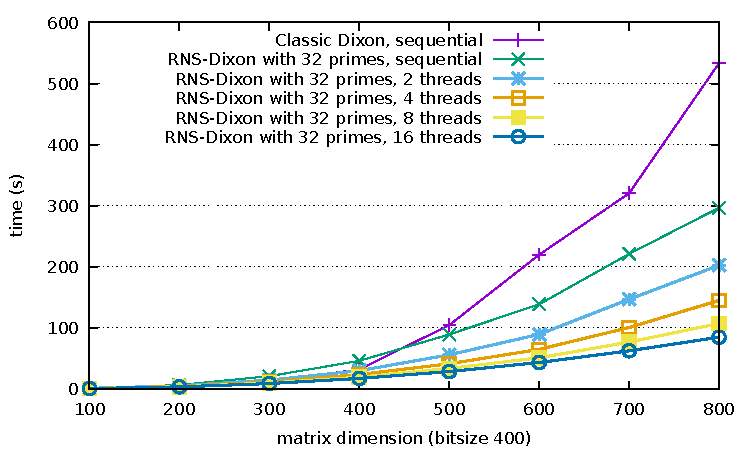
\includegraphics[width=.8\textwidth]{Pictures/RNSDixon/parallel-threads}
\end{center}
\caption{Parallel RNS Dixon.}\label{fig:rnsdixon_parallel_threads}
\end{figure}

\begin{figure}[htb]
\begin{center}
  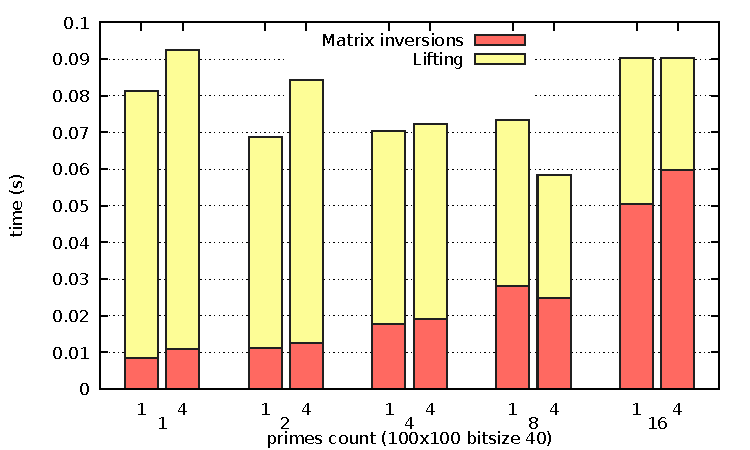
\includegraphics[width=.8\textwidth]{Pictures/RNSDixon/parallel-detailed_100n_40b}
  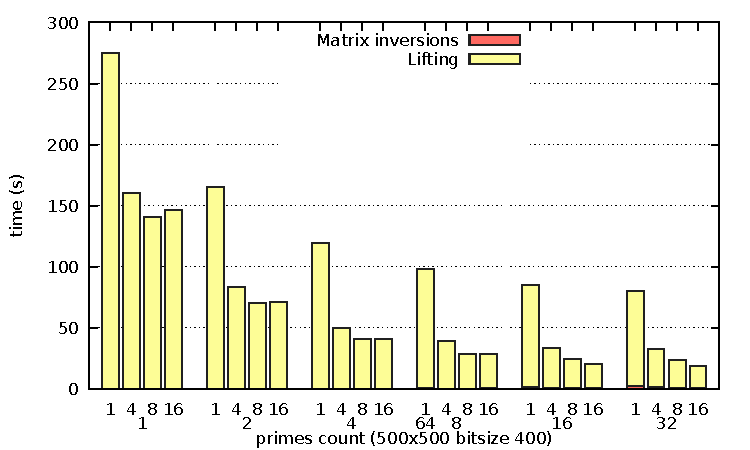
\includegraphics[width=.8\textwidth]{Pictures/RNSDixon/parallel-detailed_500n_400b_total}
\end{center}
\caption{Balance between matrix inversion (INV) and lifting phases
  (MVmod+MMZ). In each cluster, leftmost column correspond to a
  sequential run, then to $4$ and $8$ cores andwith the rightmost
column to a run with $16$ cores}\label{fig:rnsdixon_parallel}
\end{figure}

Further work is required to tune up at a finer grain the different
levels of parallelism used in the large precision RNS matrix-matrix
multiplication or to automatically deduce the right choice of
parameter $\ell$ from the characteristics of the matrix and the right
hand side.

%%%%%%%%%%%%%%%%%%%%%%%%%%%%%%%%%%%%%%%%%%%%%%%%%%%%%ùù
\subsection{GPU enabled libraries}

Graphic Processing Unit (GPU) have become a widespread component in modern high performance computing plateforms. They
offer a very high computing throughput for a contained power consumption but only for applications well suited for their
constraints:
\begin{itemize}
\item the GPU has its own onboard memory and thus data transfer from and to the main memory are expensive and may
  quickly become a bottleneck
\item the type of computation must be very regular (same code kernel applied to multiple sets of data) with as few
  branching and control instructions as possible.
\end{itemize}

Matrix multiplication is among these applications which can easily benefit from the power of GPUs. Other computations
such as Gaussian elimination, require branching, data permutations, divisions and other operations much less suited for
GPUs and therefore require communications back and forth between the main memory and the GPU memory.

Nvidia provides a set of BLAS routines, for dense linear algebra of floating point numbers, supporting their GPUs in the
library CUBLAS.

The \texttt{fflas-ffpack} library aims at providing a similar set of routines over a finite field by relying exploiting a
numerical BLAS under the hood. In this first attempt at supporting GPU's for finite field linear algebra, we therefore
focused on interfacing CUBLAS in the \texttt{fflas-ffpack} library so that matrix multiplication over a finite field
could benefit from CUBLAS' routines.

The user of the library only need to specify at configure time a path where a CUDA library is installed:
\begin{verbatim}
$> ./configure --with-cuda=/applis/dahu/cuda/cuda-10.0/lib64
\end{verbatim}

He can then transparently run his code and benefit from the speedup of the BLAS library. Figure~\ref{fig:fgemm_gpu}
shows the computation speed achieved on an NVIDIA Tesla V100 GPU, compared to the existing multi-core parallel
implementation and the sequential implementation.

\begin{figure}[htb]
\begin{center}
  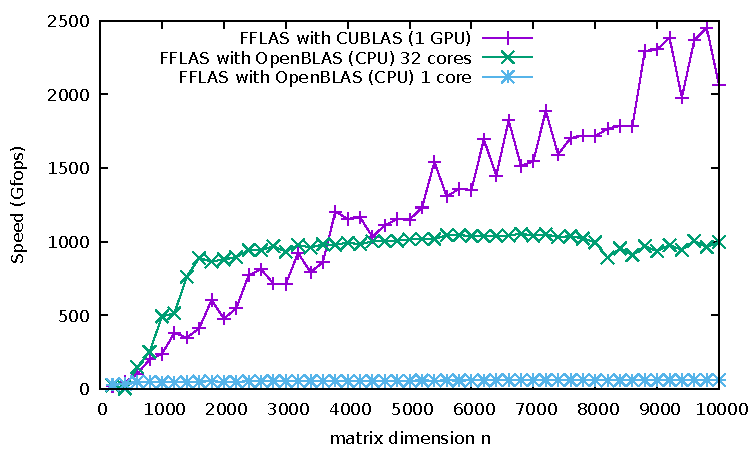
\includegraphics[width=.9\textwidth]{Pictures/fgemm_GPUvsCPU}
\end{center}
\caption{Computation speed of FFLAS-FFPACK matrix product over $\mathbb{Z}/131071\mathbb{Z}$ on a server with 1 NVidia  Tesla V100 GPU, and 32 Intel Xeon Gold 6130 cores.}\label{fig:fgemm_gpu}
\end{figure}
The speed-up of one GPU with respect to the sequential implementation is up to a factor 39.5 and up to 2.46 with respect
to a parallel execution on 32 cores.

Note that the efficiency of the GPU runs is slowly increasing and therefore perform slower than the multicore
implementation on smaller dimensions. This is due to the communication  time spent in transfering the data to and from
the GPU. This overhead is quadratic in the matrix dimension and thus becomes negligeable compared to as the dimension
increases.

This is the reason why other routines relying on many matrix multiplication, such as Gaussian elimination, matrix
inverse, etc, cannot blindly benefit from the efficiency of this matrix multiplication routine. Further work will
consist in implementing dedicated finite field Gaussian elimination routines on the GPU, and/or exploring the various
techniques to schedule the memory transfer so that they overlap with computation.

\bibliographystyle{plainnat}
\bibliography{D5.14}


%%% Local Variables:
%%% mode: latex
%%% mode: flyspell
%%% ispell-local-dictionary: "american"
%%% TeX-master: "report"
%%% End:
